\newcommand{\myparagraph}[1]{\paragraph{#1}\mbox{}\\}

\chapter{Risorse, Design UI e Networking}

\section{Risorse}

Un'applicazione è composta dal codice e dalle \textbf{risorse}, ossia tutto ciò
che non è codice (es. file del layout in XML, pacchetti delle lingue, immagini,
audio, video, ecc).
Ci sono degli ottimi motivi per utilizzare le risorse:

\begin{itemize}
\item Separare la rappresentazione dei dati (\textit{layout}) dalla gestione dei
dati (\textit{logica});
\item Fornire risorse alternative per supportare le configurazioni specifiche
dei dispositivi (es. lingua);
\item Ricompilare solo quando è strettamente necessario.
\end{itemize}

\subsection{Eterogeneità dei dispositivi}

Un'applicazione Android può essere eseguita su dispositivi eterogenei con
caratteristiche differenti (es. dimensioni dello schermo, lingua, tipo di
tastiera, ecc). Ci sono due differenti approcci a questo problema, quello
tradizionale e quello implementato in Android.
L'approccio tradizionale prevede di inserire tutte le possibilità nel codice,
per cui sarà pieno di casi \emph{if-then-else}. Per questo motivo,
l'applicazione deve essere ricompilata ogni volta che viene effettuata una
modifica (es. cambio di layout, aggiunta di una lingua).
L'approccio utilizzato in Android prevede di separare il codice dalle risorse,
usando un approccio dichiarativo basato su XML per definire le risorse stesse.
Nella Figura~\ref{img:lab2-fig1} possiamo osservare un esempio di come il codice
in Java venga separato dalle varie risorse.

\begin{figure}[htbp]
        \centering
        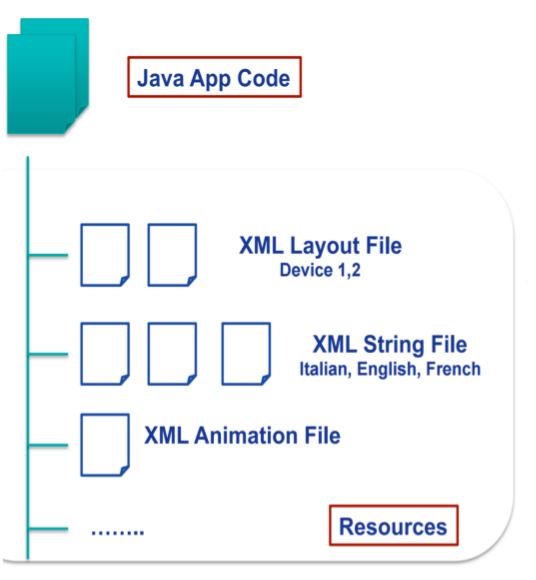
\includegraphics[width=0.3\textwidth]{lab2-fig1}
        \caption[Esempio di separazione tra codice e risorse]{Esempio di
separazione tra codice e risorse.}\label{img:lab2-fig1}
\end{figure}

\subsubsection{Approccio Android}

Gli step che prevede questo metodo sono:

\begin{enumerate}
\item Usare file XML per definire;
\begin{itemize}
\item Layout dell'applicazione;
\item Testo usato nell'applicazione;
\item Menù dell'applicazione;
\item Animazioni;
\item Alcuni esempi si trovano nella Figura~\ref{img:lab2-fig2};
\end{itemize}
\item Prevedere differenti risorse per configurazioni differenti dei vari
dispositivi;
\item Costruire il layout tramite file XML o l'editor;
\item Definire layout XML differenti per dispositivi differenti;
\item A run-time, il \textit{sistema Android} rileva la configurazione del
dispositivo (\textit{locale}) e carica le risorse appropriate (in questo modo
non è necessario ricompilare);
\item Aggiungere nuovi file XML per supportare nuovi dispositivi.
\end{enumerate}

\begin{figure}[htbp]
        \centering
        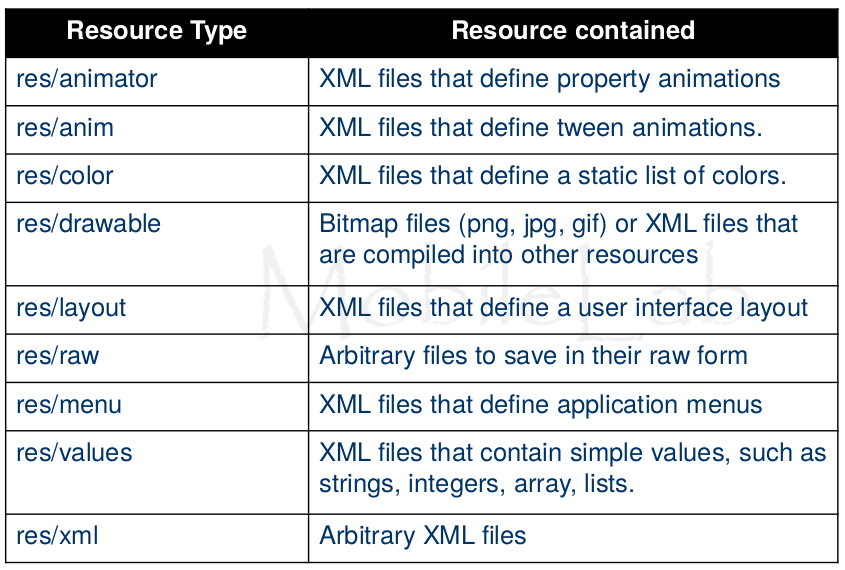
\includegraphics[width=0.8\textwidth]{lab2-fig2}
        \caption[Elenco risorse]{Un breve elenco delle risorse utilizzate sotto
forma di file XML.}\label{img:lab2-fig2}
\end{figure}

Le risorse vengono definite con un approccio dichiarativo attraverso
\texttt{XML}: ogni risorsa ha un \textit{nome/identificatore}.

\lstinputlisting[language=XML]{res/code/lab2-es1.xml}

Le risorse possono essere accedute dal codice \texttt{Java} tramite la classe
\texttt{R} (Risorse), che funge da collegamento tra il mondo di \texttt{Java} e
quello delle risorse, contendo tutti gli identificativi delle risorse nella
cartella \texttt{res/}. Viene generata automaticamente (nessuna necessità di
modificarlo) e viene rigenerato in caso di modifiche nella directory
\texttt{res/}.

Ogni risorsa ha associato un ID univoco, che è composto da due parti:
\begin{itemize}
\item il \textit{tipo} della risorsa (e.g. \texttt{String}, \texttt{int})
\item il \textit{nome} della risorsa, che può essere il \textit{nome del file},
escludendo l'estensione, oppure il valore nell'attributo \texttt{XML
<android:name>}
\end{itemize}

Le risorse possono essere accedute in due modi: tramite file \texttt{XML} o dal
codice \texttt{Java}.

\myparagraph{Accesso tramite XML}


\begin{lstlisting}[language=XML]
@[<package_name>:]<resource_type>-<resource_name>
\end{lstlisting}

\texttt{<package\_name>} è il nome del package nel quale la risorsa è collocata
(non necessario quando ci si riferisce a risorse dello stesso package).

\texttt{<resource\_type>} è il nome del tipo di risorsa.

\texttt{<resource\_name>} può essere il nome del file della risorsa (senza
estensione) o il valore dell'attributo \texttt{android:name}

\begin{figure}[htbp]
        \centering
        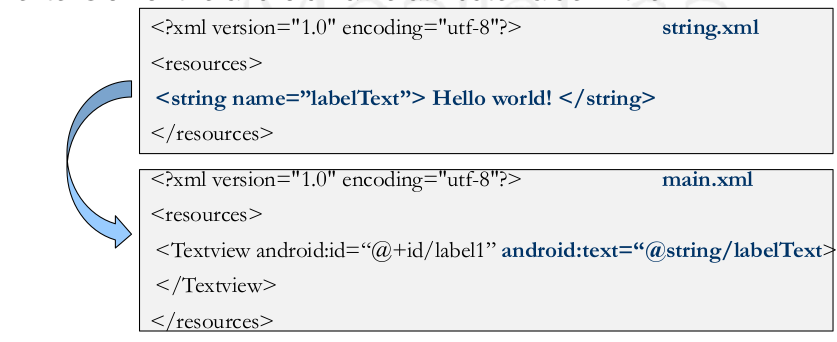
\includegraphics[width=0.7\textwidth]{lab2-fig3}
        \caption[Accesso Risorse XML]{Esempio di accesso a risorse tramite
codice XML}\label{img:lab2-fig3}
\end{figure}

\myparagraph{Accesso tramite Java}

\begin{lstlisting}[language=Java]
[<package_name>.]R.<resource_type>.<resource_name>
\end{lstlisting}

\begin{figure}[htbp]
        \centering
        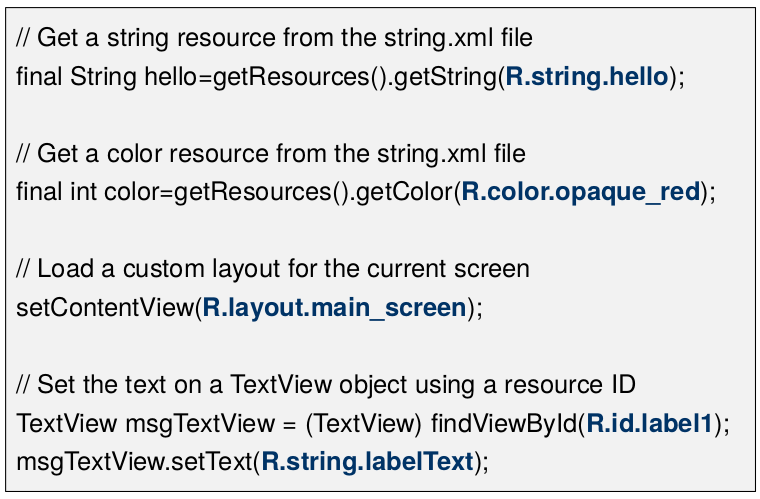
\includegraphics[width=0.6\textwidth]{lab2-fig4}
        \caption[Accesso Risorse Java]{Esempio di accesso a risorse tramite
codice Java}\label{img:lab2-fig4}
\end{figure}

\subsection{Risorse alternative}

Le applicazioni Android possono fornire delle risorse alternative per supportare
configurazioni differenti di dispositivi. A runtime, Android rileva qual è la
configurazione corrente del dispositivo e carica le risorse appropriate per
l'applicazione. Per specificare le risorse alternative:

\begin{itemize}
\item creare una nuova cartella in \texttt{res/}, scegliendo il nome con il
formato \\ \texttt{<resource\_name>-<config\_qualifier>},dove:
\begin{itemize}
\item \texttt{<resource\_name>} è il nome della cartella corrispondente alle
risorse di default;
\item \texttt{<config\_qualifier>} è il nome che specifica una particolare
configurazione per cui le risorse devono essere utilizzate;
\end{itemize}
\item salvare le risorse alternative nella nuova directory.
\end{itemize}

\begin{figure}[htbp]
        \centering
        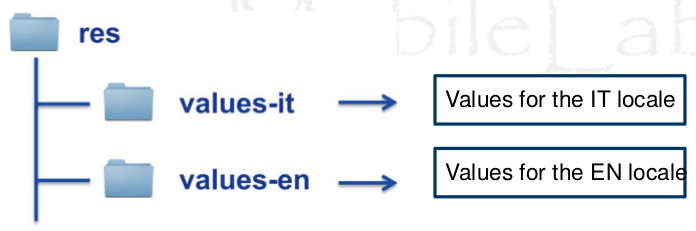
\includegraphics[width=0.7\textwidth]{lab2-fig5}
        \caption[Risorse alternative]{Esempio di distinzione delle
risorse.}\label{img:lab2-fig5}
\end{figure}

\subsubsection{Qualificatori}

Alcuni dei possibili qualificatori vengono elencati nella
Figura~\ref{img:lab2-fig6}.

\begin{figure}[htbp]
        \centering
        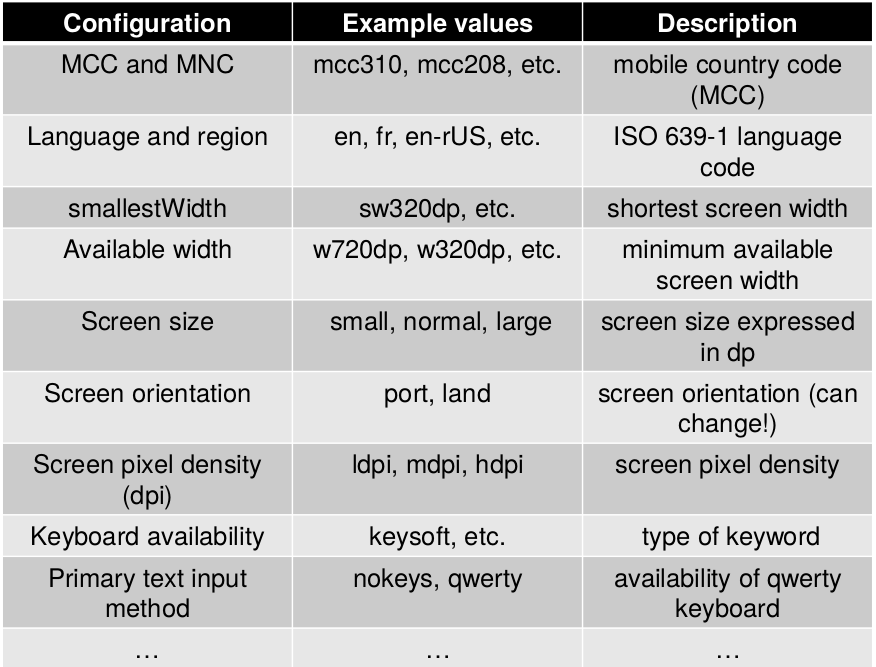
\includegraphics[width=0.8\textwidth]{lab2-fig6}
        \caption[Qualificatori]{Un breve elenco dei possibili
qualificatori.}\label{img:lab2-fig6}
\end{figure}

\subsubsection{Matching}

Quando un'applicazione richiede una risorsa che ha più alternative, il sistema
Android seleziona quale alternativa utilizzare a runtime a seconda della
configurazione del dispositivo seguendo l'algoritmo della
Figura~\ref{img:lab2-fig7}.

\begin{figure}[h]
        \centering
        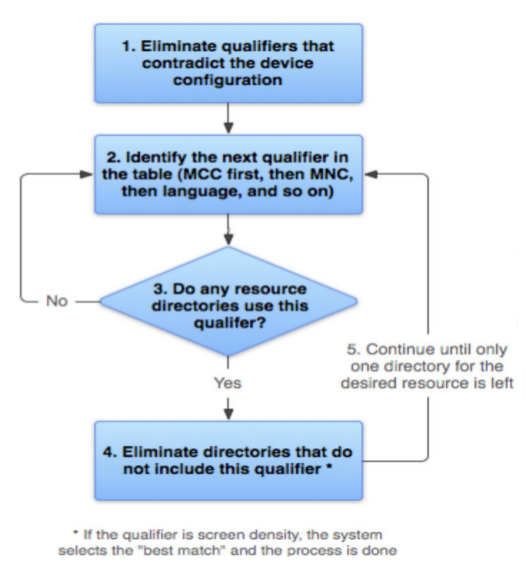
\includegraphics[width=0.6\textwidth]{lab2-fig7}
        \caption[Flowchart Risorse]{Diagramma di flusso per la scelta delle
risorse da utilizzare}\label{img:lab2-fig7}
\end{figure}

Per esempio, prendiamo la seguente configurazione di un dispositivo:
\begin{itemize}
\item \texttt{Locale = it}
\item \texttt{Screen orientation = port}
\item \texttt{Screen pixel density = hdpi}
\item \texttt{Touchscreen type = notouch}
\item \texttt{Primary text input method = 12 key}
\end{itemize}

avendo a disposizione le seguenti risorse

\begin{enumerate}
\item \texttt{drawable/}
\item \texttt{drawable-it/}
\item \texttt{drawable-fr-rCA/}
\item \texttt{drawable-it-port/}
\item \texttt{drawable-it-notouch-12key/}
\item \texttt{drawable-port-ldpi/}
\item \texttt{drawable-port-notouch-12key/}
\end{enumerate}

Utilizzando l'algoritmo, eliminiamo prima le opzioni 1, 3, 6, 7; successivamente
2 e 5, rimanendo come unica opzione la configurazione 4.

\section{Componenti della UI}

In Android tutti gli elementi dell'interfaccia utente sono costruiti utilizzando
gli oggetti \texttt{View} e \texttt{ViewGroup}.

\texttt{View}: oggetto che disegna qualcosa sullo schermo con cui l'utente può
interagire (es. un bottone).
\texttt{ViewGroup}: oggetto (contenitore) che contiene altri oggetti
\texttt{View} (o \texttt{ViewGroup}) per definire il layout dell'interfaccia
utente.

\begin{figure}[htbp]
        \centering
        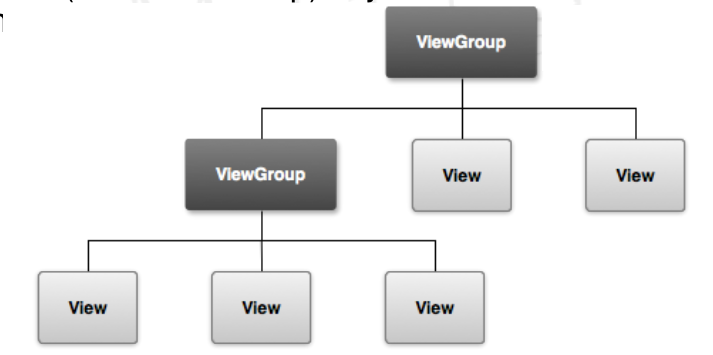
\includegraphics[width=0.5\textwidth]{lab2-fig8}
        \caption[Gerarchia View]{Gerarchia delle
\texttt{View}}\label{img:lab2-fig8}
\end{figure}

La \texttt{ViewGroup} è un contenitore vuoto delle \texttt{View} figlie:
\begin{itemize}
\item le \texttt{View} figlie possono essere controlli per l'input o widget che
disegnano componenti dell'interfaccia utente;
\item l'albero delle gerarchie può essere complesso/semplice a seconda delle
esigenze;
\item gli alberi semplici sono i migliori per le performance.
\end{itemize}

\begin{figure*}[htbp]
        \centering
        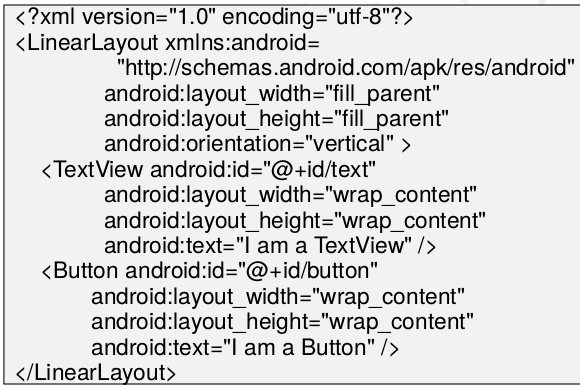
\includegraphics[width=0.5\textwidth]{lab2-fig9}
        \caption[LinearLayout]{Esempio di \texttt{LinearLayout}}
        \label{img:lab2-fig9}
\end{figure*}

Il \texttt{LinearLayout} è una \texttt{ViewGroup} che specifica come gli
elementi della UI sono posizionati a run-time. \texttt{TextView} e
\texttt{Button} sono \texttt{View} particolari chiamate \texttt{Widget}, ossia
delle \texttt{View} in miniatura che possono essere incorporate dentro ad altre
applicazioni.

Tutti i layout devono estendere la classe \texttt{ViewGroup}. Ogni \texttt{View}
deve specificare le sue dimensioni attraverso gli attributi 
\texttt{android:layout\_height} e \texttt{android:layout\_width}, che possono
essere valorizzati con:
\begin{itemize}
\item un valore numerico espresso in \texttt{dp} (o \texttt{px}), ad esempio 
\texttt{20dp};
\item \texttt{match\_parent} la \texttt{View} diventa grande
quanto il suo contenitore gli permette di espandersi;
\item \texttt{wrap\_content} la \texttt{View} imposta la
propria dimensione in base alla dimensione del suo contenuto.
\end{itemize}

I layout possono essere posizionati dentro ad altri layout. Alcuni sono
predefiniti da Android:

\begin{itemize}
\item \texttt{LinearLayout}: tutti i figli vengono organizzati in una singola
direzione, orizzontale o verticale;
\item \texttt{RelativeLayout}: mostra i figli nelle posizioni relative;
\item \texttt{TableLayout}: mostra i figli in righe e colonne;
\item \texttt{FrameLayout}: progettato per bloccare un'area sullo schermo per
mostrare un singolo elemento.
\item ....
\end{itemize}

\subsection{Caricare XML}

Quando un'applicazione viene compilata ogni file \texttt{XML} del layout viene
compilato diventando una risorsa \texttt{View}, la quale è accessibile tramite
il suo identificatore attraverso la classe \texttt{R}.

\begin{figure*}[htbp]
        \centering
        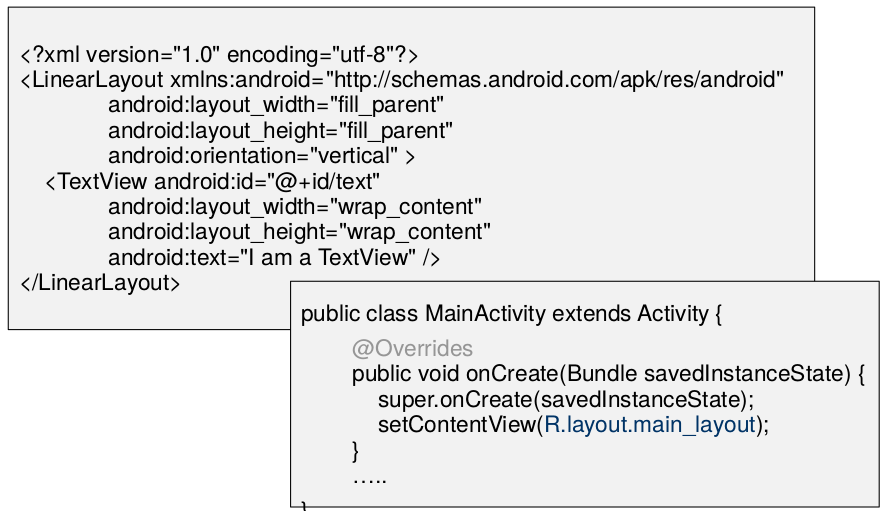
\includegraphics[width=0.75\textwidth]{lab2-fig10}
        \caption[Accesso risorse R]{Accesso delle risorse tramite la classe
\texttt{R}}
        \label{img:lab2-fig10}
\end{figure*}

\subsubsection{Stili e temi}

I \textit{temi} sono il meccanismo di Android per applicare uno stile
consistente ad un'applicazione o ad una \texttt{Activity}. Lo \textit{stile}
specifica le proprietà visive degli elementi che formano l'interfaccia utente
(es. colore, dimensione del font, ecc).
Android fornisce almeno tre temi di sistema che possono essere utilizzati
durante lo sviluppo dell'app: material (versione dark), material light (versione
light) e material light con la action bar dark. Il tema viene specificato in
\texttt{res/style}

\begin{lstlisting}[language=XML]
<resources>
    <style name="AppTheme" parent="android:Theme.Material" />
</resources>
\end{lstlisting}

\subsection{Densità dello schermo, dimensioni e layout}

Unità da conoscere:
\begin{itemize}
\item \texttt{dp} o \texttt{dip} significa pixel indipendenti dalla densità
\textit{density-independent pixels};
\item \texttt{dpi} o \texttt{ppi} significa punti (\textit{dots}) o pixel per
pollice (\textit{inch});
\item \texttt{px} significa pixels. Un pixel occupa un quantitativo arbitrario di spazio
sullo schermo a seconda della densità;
\item la relazione è data dalla formula: $px = dp * (dpi/160)$
\end{itemize}

Android raggruppa tutte le effettive densità degli schermi in 6 densità
generalizzate:

\begin{enumerate}
\item bassa densità (ldpi) $\approx$ 120 dpi
\item media densità (mdpi) $\approx$ 160 dpi
\item alta densità (hdpi) $\approx$ 240 dpi
\item extra alta densità (xdpi) $\approx$ 320 dpi
\item densità extra extra alta (xxhdpi) $\approx$ 480dpi
\item densità extra extra extra alta (xxxhdpi) $\approx$ 640 dpi
\end{enumerate}

\subsubsection{Supportare più schermi}

Bisogna specificare nel manifest quali dimensioni di schermo sono supportate
dall'applicazione, tramite l'attributo \texttt{<support-screens>} che
sovrascrive e ridefinisce alcuni comportamenti dell'algoritmo di matching di
default.
Inoltre, è necessario fornire layout differenti a seconda della dimensione dello
schermo (usando i qualificatori per specificare quale deve essere utilizzato).
Da Android 3.2 per specificare la minima larghezza disponibile si utilizza
\texttt{sw<N>dp}.
Infine, devono essere forniti bitmap differenti a seconda della densità dello
schermo: di default, Android scala i bitmap disegnabili, creando potenziali
artefatti nell'immagine. I qualificatori per la risorsa
\texttt{density-specific} sono ldpi, mdpi, ecc.

\subsection{Costruire layout con un Adapter}

L'\texttt{Adapter} viene utilizzato quando il contenuto del layout è dinamico o
non pre-determinato; popola il layout con le \texttt{View} a runtime, una
sottoclasse della classe \texttt{AdapterView} usa un \texttt{Adapter} per
collegare i dati al loro layout, fungendo da ponte tra la fonte dei dati e il
layout \texttt{AdapterView}. In pratica, l'\texttt{Adapter} recupera i dati (da
una fonte come un array o un database) e converte ogni elemento in una
\texttt{View} che può essere aggiunta al layout \texttt{AdapterView}.
I più comuni layout supportati dagli \texttt{Adapter} sono: \texttt{ListView} e
\texttt{GridView}.

\subsubsection{Come funziona}

Gli step sono:

\begin{enumerate}
\item inizializzare l'\texttt{Adapter};
\item legare l'adapter alla \texttt{ListView};
\item ottenere un riferimento alla \texttt{ListView} (n.b. visto che estendiamo
una \texttt{ListActivity} abbiamo una \texttt{ListView}, non ci serve trovare un
riferimento a quest'ultima nella gerarchia, basta il metodo
\texttt{getListView()});
\item settare \texttt{onClickListener} sulla \texttt{ListView}.
\end{enumerate}

\begin{lstlisting}[language=Java]
ArrayAdapter<String> mAdapter = new ArraryAdapter<>(this,
R.layout.listview_layout, FACULTY); //inizializzare
setListAdapter(mAdapter); //collegare
ListView listView = getListView(); //ottenere riferimento
listView.setOnClickListener(mListener); //settare il listener
\end{lstlisting}

\subsection{Shared Preferences}

Android fornisce i servizi di accesso alla memoria per: (i) mantenere i dati di
cui l'app può avere bisogno in seguito e (ii) condividere dati tra le varie app.
Ci sono differenti opzioni: usare le \texttt{SharedPreferences} per dati
semplici come \texttt{int}, \texttt{String}, ecc; usare la memoria
interna/esterna del dispositivo o usare un database \texttt{SQLite} per salvare
dati strutturati.
Le \texttt{SharedPreferences} vengono quindi utilizzate per salvare dati di 
\textit{piccole dimensioni} in un file come coppie \textit{chiave-valore}. 
Questi dati possono essere condivisi con altre app.

\subsection{Fragments}

I \texttt{Fragment} sono parti della UI dell'applicazione o comportamenti che
vengono integrati nelle \texttt{Activity}; di conseguenza un \texttt{Fragment}
necessita di una \texttt{Activity} per essere eseguito. Possono essere
considerati come delle piccole \texttt{Activity} molto leggere.
Sono componenti \textit{flessibili} e \textit{riusabili} definiti dal
programmatore, progettati per il riuso; evitare di manipolare un
\texttt{Fragment} da un altro \texttt{Fragment}. Presentano una interfaccia
utente consistente in applicazioni e dispositivi differenti, permettendo di
adattare l'esperienza dell'utente in ambienti differenti (smartphone, tablet,
ecc).
Ogni \texttt{Fragment} ha il proprio ciclo di vita, che è associato alla UI. Per
decidere quanti utilizzarne si usa la \textit{regola del pollice}: uno per ogni
tipo di dato che viene visualizzato (es. preferenze, profilo, mappa, ecc) o per
input dell'utente.

\begin{figure}[htbp]
        \centering
        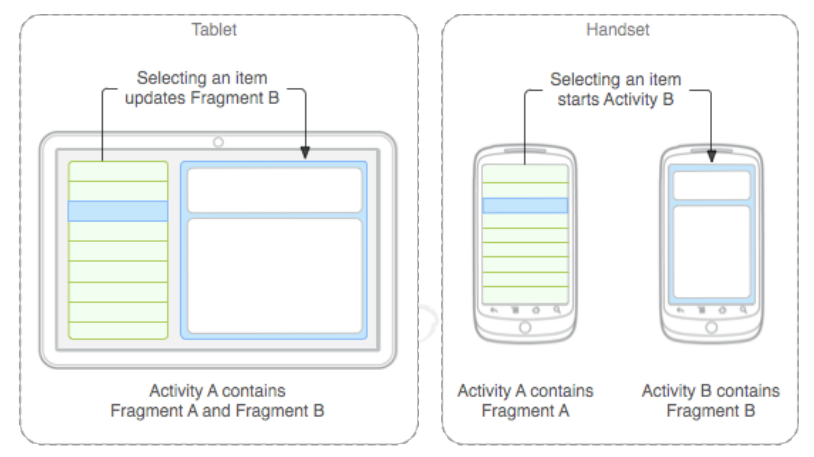
\includegraphics[width=0.7\textwidth]{lab2-fig12}
        \caption[Fragment Tablet Smartphone]{Differenze di utilizzo di un
\texttt{Fragment}}\label{img:lab2-fig12}
\end{figure}

A sinistra viene mostrato un tablet dove il \texttt{main\_activity\_layout.xml}
contiene due \texttt{Fragment} collegati all'\texttt{Activity A}. A destra c'è
un dispositivo il cui schermo non permette di visualizzare entrambi i
\texttt{Fragment}, di conseguenza vengono collegati ad \texttt{Activity}
differenti.

Per aggiungere o rimuovere \texttt{Fragment}, è necessario un riferimento al
\texttt{FragmentManager}. Queste operazioni vengono chiamate
\textit{transazioni} sulla Android Platform.

\subsubsection{Ciclo di vita di un Fragment}

\begin{figure}[htbp]
        \centering
        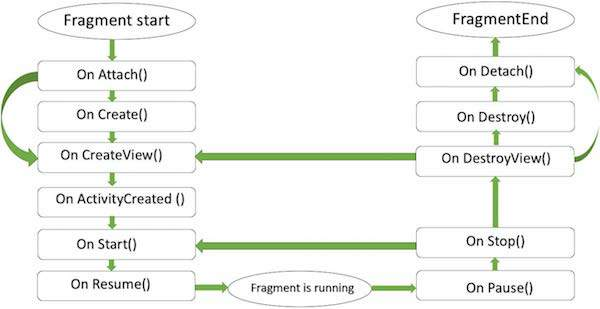
\includegraphics[width=0.7\textwidth]{lab2-fig13}
        \caption[Ciclo di vita Fragment]{Ciclo di vita di un
\texttt{Fragment}}\label{img:lab2-fig13}
\end{figure}

\begin{enumerate}
\item \texttt{onAttach()} viene chiamato quando un \texttt{Fragment} viene
collegato alla sua \texttt{Activity}
\item \texttt{onCreate()} viene chiamato per creare il \texttt{Fragment},
inizializzando le componenti essenziali per quando il \texttt{Fragment} viene
avviato o messo in pausa e poi richiamato.
\item \texttt{onCreateView()} viene chiamato per creare la sua UI. Per disegnare
una UI per il \texttt{Fragment}, bisogna ritornare da questo metodo una
\texttt{View} che è la radice del layout del \texttt{Fragment}. Si può ritornare
\texttt{null} se il \texttt{Fragment} non possiede una UI;
\item \texttt{onStart()} viene chiamato all'inizio del tempo di vita in cui è
visibile. Qualsiasi modifica alla UI può essere eseguita prima che il
\texttt{Fragment} sia visibile;
\item \texttt{onResume()} viene chiamato all'inizio del ciclo di vita attivo, in
modo da riprendere ogni aggiornamento all'UI che era in pausa e sospeso da quando
è diventato inattivo;
\item \texttt{onPause()} è la prima indicazione che l'utente sta abbandonando il
\texttt{Fragment}, anche se questo non significa che stia per essere distrutto.
Questo è il momento per salvare qualsiasi cambiamento che deve essere
persistente oltre la corrente sessione utente
\end{enumerate}


\subsection{AsyncTask}

Visto che una \texttt{Activity} è un flusso singolo di esecuzione che viene
lanciato sul thread dell'UI, i metodi del ciclo di vita della \texttt{Activity}
hanno una transizione rapida e non possono contenere operazioni pesanti che
blocchino la UI; questo genere di task devono essere tenuti fuori dal thread
della UI.
Gli \texttt{AsyncTask} permettono un uso appropriato e semplificato dei thread
dell'interfaccia utente: permettono di effettuare operazioni in background e
pubblicare i risultati sul thread della UI senza dover manipolare direttamente i
thread; non costituiscono un framework generico per la gestione dei thread e
devono essere usati idealmente per operazioni brevi (in alternativa usare
\texttt{Executor}, \texttt{ThreadPoolExecutor} e \texttt{FutureTask}).

\begin{figure}[htbp]
        \centering
        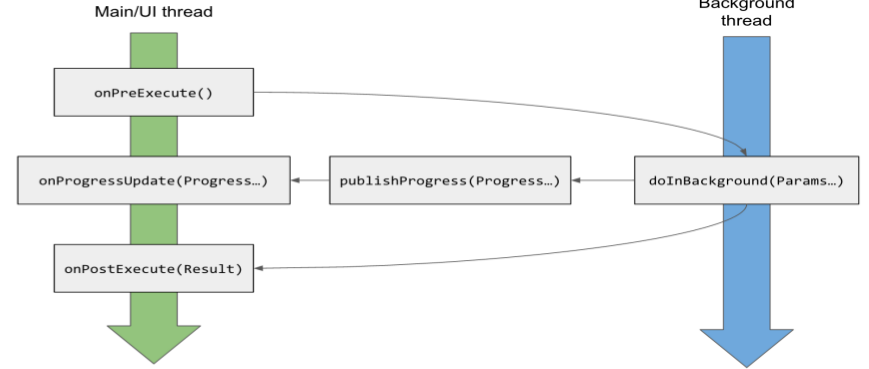
\includegraphics[width=0.7\textwidth]{lab2-fig14}
        \caption[Esecuzione AsyncTask in Fragment]{Esecuzione di un
\texttt{AsyncTask}}\label{img:lab2-fig14}
\end{figure}

\begin{itemize}
\item \texttt{onPreExecute()} viene invocato sul thread della UI prima che il
task venga eseguito. Di solito questo passo viene utilizzato per fare il setup
del task, per esempio mostrando una barra di progresso sulla UI dell'utente;
\item \texttt{doInBackground()} viene invocato sul thread in background subito
dopo che \texttt{onPreExecute()} ha finito di eseguire. Questo step viene usando
per effettuare le computazioni in background che possono richiedere molto tempo.
Può richiamare il metodo \texttt{publishProgress()} per aggiornare la UI a
seconda del progresso dell'operazione;
\item \texttt{onProgressUpdate()} viene invocato sul thread dell'UI dopo una
chiamata a \texttt{publishProgress()}. Il tempo per l'esecuzione è indefinito;
\item \texttt{onPostExecute()} viene chiamato sul thread della UI dopo che la
computazione in background ha terminato. Il risultato della computazione viene
passato a questo step tramite un parametro.
\end{itemize}

\subsubsection{Come funziona}

Segue un esempio di un'applicazione che effettua un countdown partendo da 15,
aggiornando la UI ad ogni cambiamento.

\begin{figure*}[htbp]
        \centering
        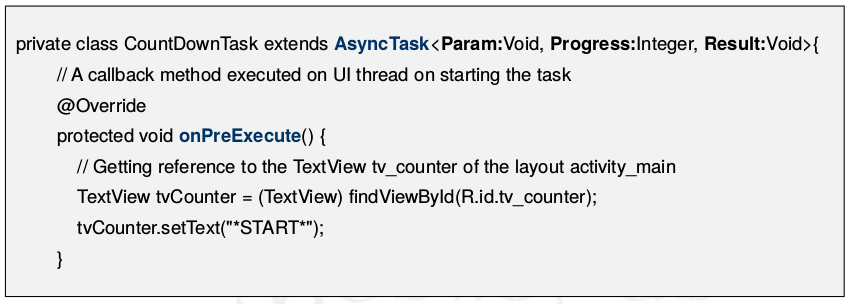
\includegraphics[width=0.7\textwidth]{lab2-fig15}
        \caption[AsyncTask per aggiornare Fragment - 1]{Esempio di utilizzo di
un \texttt{AsyncTask} per aggiornare un Fragment - Parte 1}
        \label{img:lab2-fig15}
\end{figure*}

Prende tre tipi come argomenti:
\begin{itemize}
\item \texttt{Params}, il tipo di parametri inviati al task durante
l'esecuzione;
\item \texttt{Progress}, il tipo di unità di progresso pubblicata durante la
computazione in background;
\item \texttt{Result}, il tipo di risultato della computazione in background.
\end{itemize}

\begin{figure*}[htbp]
        \centering
        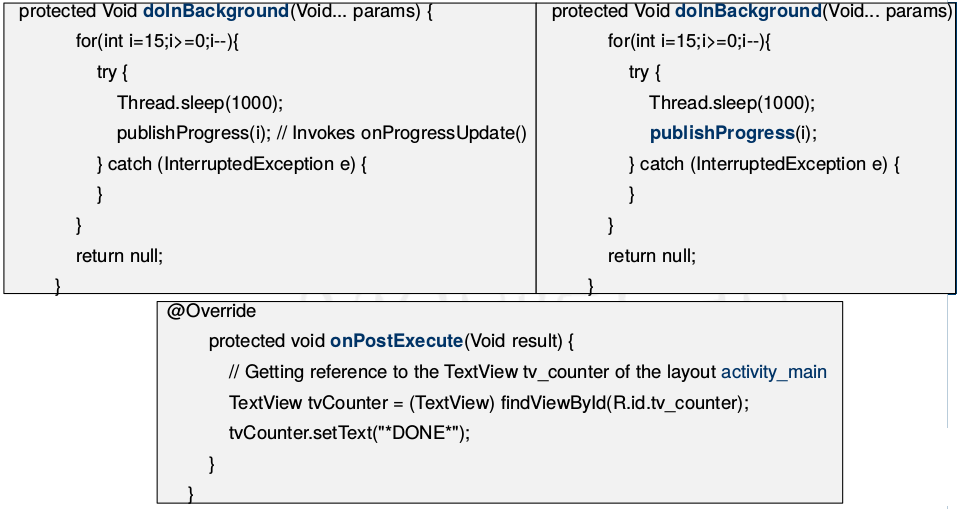
\includegraphics[width=0.7\textwidth]{lab2-fig16}
        \caption[AsyncTask per aggiornare Fragment - 2]{Esempio di utilizzo di
un \texttt{AsyncTask} per aggiornare un Fragment - Parte 2}
        \label{img:lab2-fig16}
\end{figure*}

\section{Networking in Android}

Android include diverse librerie per la programmazione della navigazione:
\begin{itemize}
\item \texttt{java.net} (\texttt{Socket} e \texttt{URL});
\item \texttt{org.apache} per richieste http (\texttt{HttpRequest},
\texttt{HttpResponse});
\item \texttt{android.net} (\texttt{URI}, \texttt{AndroidHttpClient},
\texttt{AudioStream}).
\end{itemize}

Per effettuare operazioni sulla rete è necessario specificare i permessi che
sono necessari all'applicazione nel file \texttt{AndroidManifest.xml}. Se i
permessi necessari non sono concessi, viene lanciata un'eccezione a runtime dal
sistema.

\begin{lstlisting}[language=XML]
<uses-permission android:name="android.permission.INTERNET" />
<uses-permission android:name="android.permission.ACCESS_NETWORK_STATE" />
\end{lstlisting}

\subsection{Socket}

Un socket è un endpoint software che può creare un canale di comunicazione tra
processi software. In pratica, sono un'interfaccia di programmazione per
effettuare comunicazioni attraverso la rete, infatti la libreria del client HTTP
Android utilizza i socket di \texttt{Java} per inviare e ricevere dati.


\subsection{Controllare la connessione}

\begin{figure*}[htbp]
        \centering
        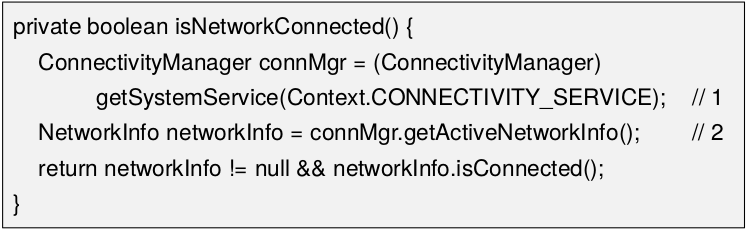
\includegraphics[width=0.7\textwidth]{lab2-fig17}
        \caption[Controllo connessione]{Controllo della connessione}
        \label{img:lab2-fig17}
\end{figure*}

\begin{enumerate}
\item \texttt{ConnectivityManager} è un oggetto che contiene lo stato della
connessione alla rete. Viene richiamato per ottenere lo stato della connessione
ma può anche notificare le applicazioni quando la connessione cambia attraverso
il meccanismo di \textit{callback};
\item Recuperare un'istanza della classe \texttt{NetworkInfo} che rappresenta
l'attuale connessione alla rete. È \texttt{null} se non c'è nessuna rete
disponibile. In questo caso un buon approccio è notificare la cosa all'utente,
la cosa può essere fatta in maniera programmatica ma deve mantenere l'utente nel
loop.
\end{enumerate}

\subsubsection{Attivare la connessione in modo programmatico}

Possiamo attivare il WiFi in maniera programmatica (senza richiedere alcun
permesso in più rispetto a prima).

\begin{lstlisting}[language=Java]
WifiManager manager = (WifiManager)
this.context.getSystemService(Context.WIFI_SERVICE);
manager.setWifiEnabled(true);
\end{lstlisting}

Prima di iniziare con le operazioni di rete abbiamo bisogno di sapere se la
connessione è disponibile; questo può avvenire tramite una notifica da parte del
sistema operativo con l'evento \texttt{CONNECTIVITY\_CHANGE} che viene inviato
in broadcast, al quale esprimiamo il nostro interesse per l'evento
(\texttt{BroadcastReceiver}).

\begin{figure*}[htbp]
        \centering
        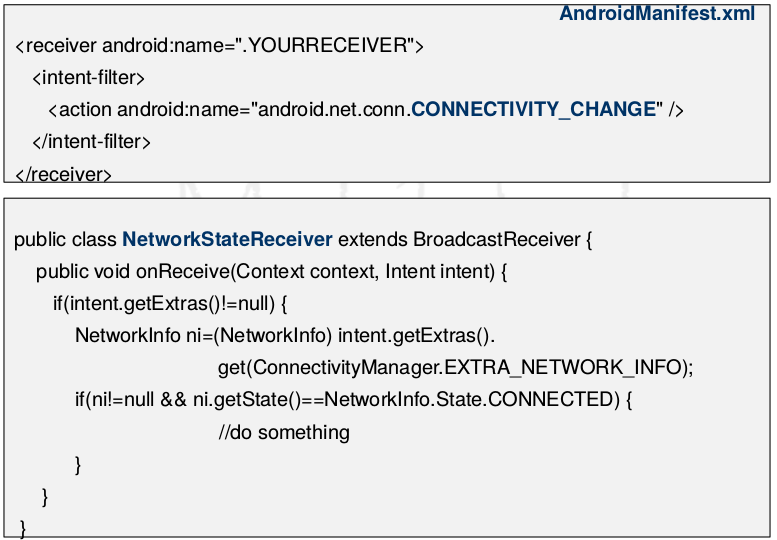
\includegraphics[width=0.8\textwidth]{lab2-fig18}
        \caption[Disponibilità rete]{Notifica disponibilità della rete}
        \label{img:lab2-fig18}
\end{figure*}

\subsection{Determinare il tipo di connessione}

Quando si ha un'applicazione che recupera un gran quantitativo di dati, è
consigliato restringere il tipo di rete ad un caso specifico, come il WiFi.
Questo può essere fatto tramite il metodo \texttt{getType()} sull'oggetto
\texttt{NetworkInfoObject} (altri tipi sono Bluetooth, Mobile, WiMax, ecc).

\subsection{Effettuare operazioni sulla rete}

Anche in questo caso, per eventi che possono rallentare la UI utilizziamo gli
\texttt{AsyncTask}.

\begin{figure}[htbp]
        \centering
        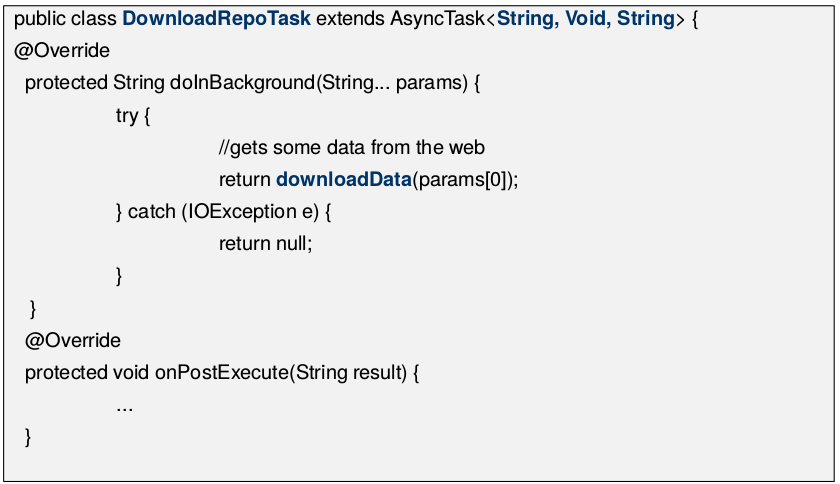
\includegraphics[width=0.7\textwidth]{lab2-fig19}
        \caption[AsyncTask sulla rete - 1]{Utilizzo di \texttt{AsyncTask} per
recuperare dati sulla rete - 1}
        \label{img:lab2-fig19}
\end{figure}

\begin{figure}[htbp]
        \centering
        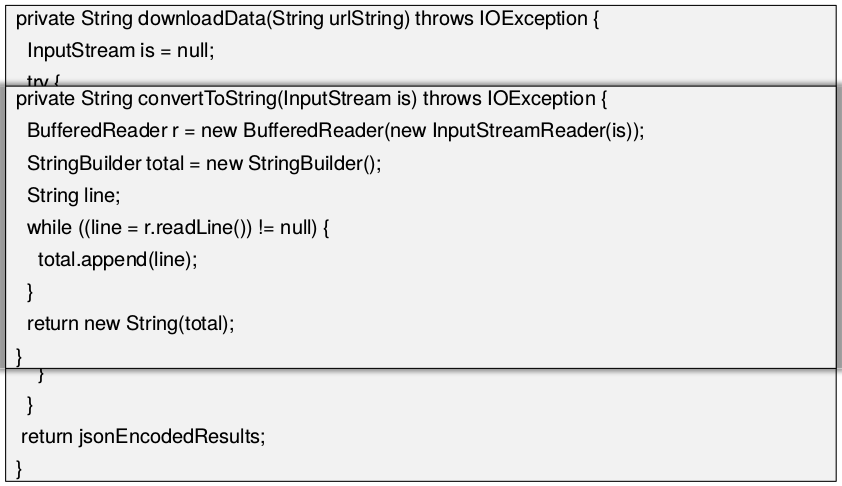
\includegraphics[width=0.6\textwidth]{lab2-fig20}
        \caption[AsyncTask sulla rete - 2]{Utilizzo di \texttt{AsyncTask} per
recuperare dati sulla rete - 2}
        \label{img:lab2-fig20}
\end{figure}

\subsection{Librerie alternative per il networking}

\begin{itemize}
\item \texttt{OkHttp}: un client Java efficiente che supporta chiamate sincrone
e asincrone. Compatibile con Android 2.3 e successivi.
\item \texttt{Volley}: è una libreria Android per effettuare chiamate rapide e
facili sulla rete, che supporta solamente chiamate asincrone. Supporta Android
1.6 e successivi.
\item \texttt{Retrofit}: è una libreria Java e Android che è molto efficiente
per recuperare informazioni strutturate come \texttt{JSON} e \texttt{XML}.
Permette di specificare una libreria per la conversione di qualsiasi dato, come
\texttt{Gson}, \texttt{Jackson}, \texttt{Moshi}, ecc.
\end{itemize}
